

 
\section{Rethinking the Problem}\label{problem}

This section suggests that detecting actionable static code warnings is a ``bumpy'' problem
(defined below) and that such problems can not be understood by learners that use simplistic
boundaries between classes.  

The core task of any classification problem is the creation of a hyperspace
boundary that let us isolate what is most desired or most interesting. Different learners build their boundaries in different ways:
\bi
\item Simple decision tree learners can only build straight-line
boundaries. 
\item Neural networks can produce very complex and convoluted boundaries.
\item And
internal to   
Kang et al.'s support vector machine was a ``radial basis function''
that allowed those algorithms to build circular hyperspace
boundaries.  
\ei 
Boundaries can be changed by adjusting
the
parameters that control the learner. For example, in Kang et al.'s radial basis functions,
the $C$ regularization parameter is used to set the tolerance of the model to (some) classifications. By adjusting $C$, an analyst can change
the generalization error; i.e. the error when the model is applied to as-yet-unseen test data.

Figure~\ref{cg} show how changes to $C$ can alter the decision
boundary between some red examples and blue examples. Note that each
setting to $C$ changes the accuracy of the predictor; i.e.
for good predictions, it is important to fit the shape of the decision boundary to the shape of the data. 

(Technical aside: while this example was based on SVM technology, the same line of argument applies to  any other classifier; i.e. changing
the control parameters of the learner also changes the hyperspace boundary 
found by that learner and, hence, the predictive prowess of that learner.)

We have tried applying    hyperparameter optimization to   $C$ in a failed attempt to improve that performance (see the C1 results of Table \ref{tab:results}). 
From that failed experiment, we conclude that   however  $C$ work
for radial bias functions, they do not work well enough to fix
the unimpressive predictive performances -- see Table~\ref{tab:initial_svm}.


 

Why do radial bias SVMs fail in this domain?  Our  conjecture is that the hyperspace boundary dividing the static code examples (into false positives and others)
is so ``bumpy''\footnote{``Bumpy'' data 
  contain complexities such
as many local minima, saddle points, very flat regions,
and/or widely varying curvatures. For example, see  Figure \ref{fig:loss}.}
that the kinds of shape changes seen
in   Figure~\ref{cg} can never adequately model those  examples.

\begin{figure}[!t]
 \noindent {\footnotesize \begin{tabular}{c@{}c@{}c}
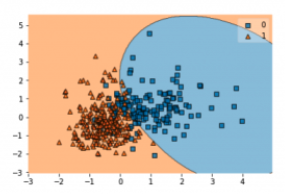
\includegraphics[height=.8in]{rahul/c0_1g0_1.png}&
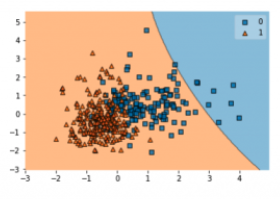
\includegraphics[height=.8in]{rahul/c0_1g0_008.png}&
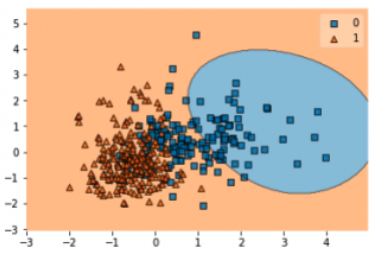
\includegraphics[height=.8in]{rahul/c0_02g_01.png}\\
$C=0.1$&$C=0.1$&$C=0.2$\\ 
$\mathit{acc}=90\%$& $\mathit{acc}=64\%$&  $\mathit{acc}=81\%$ 
\end{tabular}}

\caption{The $C$  parameter of a radial basis function alters
the shape of the hyperspace boundary.  {\em Acc} is accuracy which is the ratio of true positives plus true negatives divided by a SVM making predictions across that boundary. Example from~\cite{kumar20}.}\label{cg}
\end{figure}

To test that conjecture, we first    checked for ``bumpiness" using a technique
from \citet{li2018visualizing}. That technique
visualizes the ``error landspace'' 
(i.e. how fast small changes in the independent variables altered the error
estimation).
% The technique is in two parts:
% \bi
% \item A way to reduce N-dimensional data to two-D plot, plus a third
% dimension to represent the loss function (e.g. see Figure \ref{fig:loss}a); 
% \item
% A  statistic that Li calls ``$\beta-$smoothness''
% that measures
% the simplicity of that landscape\footnote{According to \citet{li2018visualizing}, given some error function $f$ and samples at point $x$,
% $\beta-$smoothness is defined as the maximum value of $\beta$ for which $\lVert \nabla f(x_1) - \nabla f(x_2) \rVert \leq \beta \lVert x_1 - x_2 \rVert$ under some norm (we use the $l_2$ norm), and is a measure of the smoothness of the loss surface (i.e., higher the $\beta-$smoothness, smoother the error surface).}. 
% \ei
For our TOMCAT data, Li et al.'s methods resulted in Figure \ref{fig:loss}.
There, we see a ``bumpy'' landscape
with several multiple local minima. 
% The presence   multiple minima means that, in different local  regions of the data,
% we will need different adjustments to the hyperspace boundary.  

Having confirmed that our data is ``bumpy'', our second step was to
we look  for ways to reduce that bumpiness. Initially, we attempted to use
  neural nets since that kind of learner is meant
to be able to handle complex hyperspace boundaries~\cite{WittenFH11}.
As discussed in \S\ref{sec:results}, that attempt failed even after trying
several different architectures such 
as
feedforward networks, CNN,  and CodeBERT~\cite{rumelhart1986learning,habib2018many,vaswani2017attention}
(with and without tuning learner control parameters).

Since standard neural net technology failed, we tried several   manipulation techniques for the training process, described in the next section.  

\begin{figure}[!t]
   \begin{center}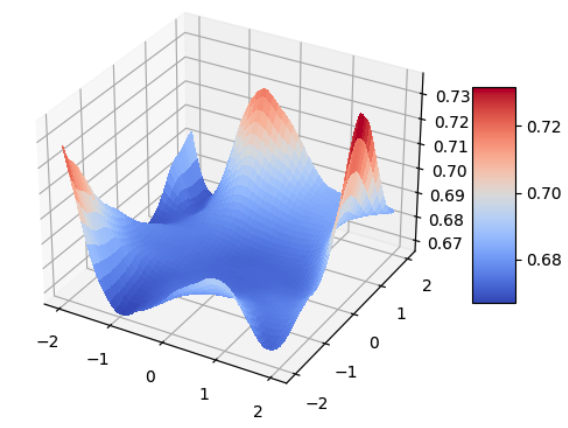
\includegraphics[width=.3\textwidth]{rahul/pre1.png} \end{center}
 
    \caption{Error landscape in the TOMCAT data    before    applying the methods of this paper. In the plot, the larger the vertical axes, the greater the loss value.
    Later in this paper,
    we will show this plot again, after it has been smoothed via the   methods of  \S\ref{rx}
    (see Figure~\ref{fig:gain} and Table~\ref{tab:fuzzy}).}
    \label{fig:loss}
\vspace{-10pt}
\end{figure}

\section{  Treatments}\label{rx}

 This section discusses a framework that holds
 operators for   treating the data in order to adjust  the decision boundary (in different ways for different parts of the data). For the purposes of illustration and experimentation,
 we offer operational examples for each part of the framework:
 \bi
 \item  SMOTE for instance engineering;
 \item  SMOOTH for label engineering;
 \item   GHOST for boundary engineering;
 \item   DODGE for parameter engineering.
 \ei
 Before presenting those parts we note here that the framework is more than just those four treatments. 
 As SE research matures, we foresee that our framework will become a workbench   within which researchers replace some/all of these treatments with more advanced options.
 
 That said, we have some evidence that  SMOTE, SMOOTH, GHOST, DODGE are useful:
 \bi
  \item
The ablation study of \S\ref{rigg}  shows that removing any one of these treatments leads to worse performance.
 \item
All these treatments are  very fast: sub-linear time for SMOTE and SMOOTH, linear time for GHOST, and DODGE is known to be orders of magnitude faster than other hyperparameter optimizers~\cite{agrawal2019dodge}.
 \ei


 

\subsection{Instance Engineering (via SMOTEing)}
To remove the ``bumpiness'' in data like Figure~\ref{fig:loss}, we need to 
pull and push the decision boundaries between different classes into a smoother shape.
But also, unlike simplistic $C$ tuning available in radial  SVMs, we want that process to perform differently
in different parts of the data.

One way to adjust the decision boundary in different parts of the data is 
to add (or delete)  artificial examples around each example $X$. This builds a little ``hill'' (or valley) in the local region.
As a result, in that local region,
 it becomes more (or less)
certain that all predictions which reach the same conclusion as $X$. In effect, adding/deleting
examples pushes the decision boundary away (or, in the case of deletions, pulls it closer).
SMOTE \cite{chawla2002smote} is one instance engineering technique that:
\bi
\item Finds  five nearest neighbors
to   $X$ with the same label;
\item  Selects one at random;
\item Creates a new example $R$, with the same label as $X$ at some random point
between $X$ and $R$.
\ei

\subsection{Label Engineering (via SMOOTHing)}

SMOTE has seen much success in recent SE papers as a way to improve predication efficacy~\cite{agrawal2018better}. 
But this technique makes a {\em linearity} assumption that all the data around $X$ is correctly labelled
(in our case, as examples of actionable or unactionable static code warnings).
This may not be true.
 \citet{cordeiro2020survey} and recent SE researchers~\cite{frugal, debtfree, 9064604, jitterbug} note that  noisy labels can occur when human annotators are present~\cite{mcnicol2005primer} or those humans  have divergent opinions about the labels~\cite{barkan2021reduce, ma2019blind}. Although our labels were re-checked by the authors of \citet{kang2022detecting}, our ablation study (below) reports that it is best to apply some
 mitigation method for 
 poorly labelled examples. For example, in this work we applied the following SMOOTHing   operator where data is assigned labels using multiple near neighbors. This has the effect of removing outliers in the data. 
 Our SMOOTH operator works as follows:
 \bi
 \item
 Given $n$ training samples (and therefore, $n$ labels), we keep $\sqrt{n}$ at random and discard the rest.
 \item
 Next, we use  a KD-tree to recursively sub-divide the remaining data into leaf clusters of   $\sqrt[4]{n}$ nearest neighbors. Within each leaf, all examples are assigned a label that is the  mode of the labels in that leaf.
 \ei
 One interesting and beneficial side-effect of SMOOTHing is that we   make conclusions on our test data using just 10\% of the training data. 
  By reducing  the labelling required to make conclusions, SMOOTHing
 offers a way to help future studies avoid the problems reported by Kang et al.~\cite{kang2022detecting}:
 \bi
 \item   One of the major finding of the Kang et al. study was that earlier work~\cite{yang2021learning}  had mislabelled much of its data. From that study, we assert that it is important for analysts to spend more time checking their labels.
 We note that there many other ways to reduce the labels required for supervised learning. 
%  In future work, we will explore {\em semi-supervised learning}~\cite{Tu21} methods, seeking ways to make conclusions using as few labels as possible.
 \item SMOOTHing reduces the effort required for that checking
 process (by a factor of ten).
 \ei
 As an aside, we note that SMOOTHing
 belongs to a class of algorithms
 called {\em semi-supervised learning}~\cite{frugal, debtfree}  that try to   make conclusions using as few labels as possible.
The literature on semi-supervised learning is voluminous \cite{berthelot2019mixmatch, fairssl, kingma2014semi,  zhai2019s4l, zhu2005semi} and so, in the theory, there could be many other better ways to perform label engineering.
This would be a productive area for future research.    But for now, the ablation
  study (reported below) shows that   SMOOTHing is useful
  (since removing it degrades predictive performance).
  

\subsection{Boundary Engineering (via GHOSTing)}

As defined above, instance and label engineering do not reflect on the quality of data in the local region.

To counter that, this study employs a boundary method called ``GHOSTing'', recently developed and applied to software defect prediction  by    \citet{yedida2021value}.
 Boundary engineering is different to label and instance engineering since it adjusts the frequency of different classes
 in the local region (while the above typically end up repeating the same label for a particular locality). Hence, in that region,
 it changes the decision boundary. 
 
 
GHOSTing addresses class imbalance issues in the data.   When an example with one label
is surrounded by too many examples of another label, then the signal associated with
example can be drowned out by its neighbors
To fix this,
for a two-class dataset $D$ with class $c_0$ being the minority, GHOSTing oversamples the class by adding concentric boxes of points around each minority sample. The number of concentric boxes is directly related to the class imbalance: higher the imbalance, more the number of boxes. Specifically, if $n$ is the fraction of samples in the minority class, then $\lfloor \log_2 (1/n) \rfloor$ boxes are added.
While the trivial effect of this is to oversample the class (indeed, as pointed out by \citet{yedida2021value}, this \textit{reverses} the class imbalance), we note that the algorithm effectively builds a wall of points around minority samples.
This pushes the decision boundary away from the training samples, which is preferred since a test sample that is close to a training sample has a lesser chance of   being
misclassified due to the decision boundary being in between
them.

Our pre-experimental intuition was that  boundary engineering would replace the need to use instance engineering. However, as shown by our ablation study, for recognizing actionable static code warnings, we needed both tools. On reflection, we realized   both may be  necessary since while (a)~boundary engineering can help make local adjustments to the decision boundary, it can (b)~only work in regions where samples \textit{exist}; instance engineering can help fill in gaps in sparser regions of the dataset.


\begin{table}[!t]
    \centering
    \caption{List of hyper-parameters tuned in our study.
    CodeBERT is not shown
  in that table since, as mentioned in the text, this analysis lacked
  the resources required to tune such a large model.}
    \label{tab:hyperparams}
    
   
    \begin{tabular}{llp{2.2cm}}
        \toprule
        \textbf{Learner} & \textbf{Hyper-parameter} & \textbf{Range}  \\
       
 \rowcolor{gray!15}         Feedforward network & \#layers & $[2, 6]$ \\
  \rowcolor{gray!15}        & \#units per layer & $[3, 20]$ \\
        
       Logistic regression & Penalty & $\{l_1, l_2\}$ \\
        & C & $\{0.1,1,10,100\}$ \\
        
  \rowcolor{gray!15}     Random forest & Criterion & $\{$ gini, entropy $\}$ \\
   \rowcolor{gray!15}       & n\_estimators & $[10, 100]$ \\
        
       Decision Tree & Criterion & $\{$ gini, entropy $\}$ \\
        & Splitter & $\{$ best, random $\}$ \\
         
  \rowcolor{gray!15}     SVM & C & $\{0.1,1,10,100\}$ \\
   \rowcolor{gray!15}       & Kernel & $\{$sigmoid, rbf, polynomial $\}$ \\
   
   CNN & \#convolutional blocks & [1, 4] \\
   & \#convolutional filters & \{4, 8, 16, 32, 64\} \\
   & Dropout probability & (0.05, 0.5) \\
   & Kernel size & \{16, 32, 64\} \\
        \bottomrule
    \end{tabular}
\end{table}
        

\subsection{Parameter Engineering (via DODGEing)}

We noted above that different learners
generate different hyperspace
boundaries (e.g. decision learners generate
straight-line borders while SVMs with radial bias functions generate circular borders). Further, once a learner
is selected, then as seen in Figure \ref{fig:loss}, 
it is possible to further adjust
a border by altering the   control parameters of
 that learner (e.g. see Figure~\ref{cg}).  We call this adjustment
 {\em parameter engineering}.
 
 Parameter engineering is like a scientist probing some phenomenon. After the data is divided into training and some
 separate test cases, parameter engineering algorithms conduct experiments on the training data looking for parameter settings
 that improve the performance of a model learned and assessed
 on the training data. Once some conclusions are
 reached about what parameters are best, then these are applied
 to the test data. Importantly, the parameter engineering  should only use the training    data for its investigations (since otherwise, that
 would be a threat to the external validity of the conclusions).
 
 
 Parameter engineering executes within the
 space of control parameters of selected learners. 
   These learners have the internal parameter space shown 
  in Table~\ref{tab:hyperparams}. 
We selected this range of learners using the following rationale:
 \bi
 \item
   In order to   compare our new results to   prior work by Kang et al. ~\cite{kang2022detecting}, we use the 
   Kang et al. {\em   SVMs}
  with the radial basis kernel and balanced class weights.
\begin{table}[!b]
    \centering
    \caption{Neural net architectures used
    in this study.}
    \label{tab:nnhere}
    
      \small
    \begin{tabular}{p{8.5cm}}
        \toprule
    \rowcolor{gray!15}
     {\em Feedforward networks}
     These are   artificial neural networks, comprising an acyclic graph of nodes that process input and produce an output. These dates back to the 1980s, and the parameters of these models are learned via backpropagation \cite{rumelhart1986learning}. 
       These networks have $\mathcal{O}(10^3)-\mathcal{O}(10^4)$ parameters. 
     For these networks, we used the    ReLU  (rectified linear activation)    function ($f(x) = \max (0, x)$).
     This is a  piecewise linear function that will output the input directly if it is positive, otherwise, it will output zero.  
        ~\\
        A {\em convolutional neural net} (CNN) is a structured neural net where the first several layers are sparsely connected in order to process information (usually visual).
        CNN is an example of an  
        {\em deep learner} and  are much larger than
        feedforward networks (these may   span $\mathcal{O}(10^5)-\mathcal{O}(10^7)$ parameters).
        Optimizing an CNN is a very complex task (so many parameters) so
        following   advice from the literature~\cite{ioffe2015batch,srivastava2014dropout}, we used the following architecture. Our CNNs had multiple ``convolutional blocks'' defined as follows:
\begin{enumerate}
    \item ReLU activation
    \item Conv (with ``same'' padding)
    \item Batch norm \cite{ioffe2015batch}
    \item Dropout \cite{srivastava2014dropout} 
\end{enumerate}

We note that this style of building convolutional networks, by building multiple ``convolutional blocks'' is very popular in the CNN literature \cite{krizhevsky2012imagenet,lecun1989backpropagation}. 
Our specific design of the convolutional blocks was based on a highly voted answer on Stack Overflow \footnote{\url{https://stackoverflow.com/a/40295999/2713263}}.

Note that with that architecture there is
still room to adjust the ordering of the blocks-- which is what we adjust when we tune our CNNs.\\   \rowcolor{gray!15} 
CodeBERT~\cite{feng2020codebert} is a {\em transformer-based}  model that been   pre-trained model using millions of examples
 from contemporary programming languages such as Python, Java, JavaScript, PHP, Ruby, and Go. 
Such transformer models
are those based on the ``self-attention'' mechanism proposed by \citet{vaswani2017attention}. CodeBERT
        is even large than CNN and can contain $\mathcal{O}(10^8)-\mathcal{O}(10^9)$ parameters.
One advantage of such large models is that can 
 learn intricacies that are missed by smaller models.   \\\bottomrule
    \end{tabular}
\end{table}    
 \item
   In order to   compare our   work to    Kang et al. ~\cite{yang2021learning}, we used 
  a range of  {\em traditional learners}
  (logistic regression, random forests, and single
 decision tree learners); 
 \item
Also, we explored the various  {\em    neural net algorithms}
shown in  Table~\ref{tab:nnhere}
since these algorithms have a reputation
 of being able to handle complex decision boundaries~\cite{WittenFH11}. 
 In this textbook on {\em Empirical
     Methods for AI}, Cohen~\cite{cohen1995empirical} advises that supposedly more complex solutions should be compared to  a range of alternatives, including very
     simple methods. Accordingly, for neural nets,
     we used (a)~feedforward networks from the 1980s;
     (b)~the CNN deep learner used in much of contemporary SE
     analytics; and (c)~the state-of-the-art   CodeBERT model.
 \ei     
% \noindent
% {\bf RQ6}  is an interesting questions since before we recommend complex algorithms,
% it is prudent to ask if that complexity is required. We say this since the cost to commission different kinds of machine learners can vary by orders of magnitude.
% For example, DODGE requires 3 seconds and 3 hours (respectively) to tune feedforward networks and CNN, respectively
% (and CODEBERT is so complex that we cannot tune it all). 
% which makes optimization difficult. To fix this, we look at prior work that successfully applied deep learning in software engineering. One such study was the GHOST study by \citet{yedida2021value}, which used a combination of hyper-parameter optimization and a novel ``fuzzy sampling'' technique. That study described the necessity of fuzzy sampling as pushing the decision boundary away from training samples so that test samples are not misclassified if they are close to a training sample, yet separated by the decision boundary. While this was convincing, we were motivated by the spirit of a study by \citet{santurkar2018does}, who showed that Batch Normalization \cite{ioffe2015batch} worked because it smoothens the surface of the loss function. Does fuzzy sampling have a similar effect? We tested this by applying fuzzy sampling as discussed by \citet{yedida2021value} and then redrawing the loss landscape. This led to Figure \ref{fig:loss}b, which is significantly smoother. We observed a similar trend across all our datasets
% its losses   loss function ss functions are   algorithm that summarizes the performance of test test. Loss functions are entire
% field of research on to themstemselves. For examle,
% the cross-entr
% non-convex. Could this non-convexity explain why these
% in the paper
% and  report here that the
% For that  purpose   (local adjustment of the separation policy), we will use {\em instance, label, boundary}
% and {\em parameter} engineering methods described in the next section.% Methods that adjusts   data   to enhance learning needs to show    that they avoid the following threat to validity:
% \bi
% \item
% A learned model must be tested on the kinds of data expected in practice (and not some artificially mutated set). 
% \iten
% Hence, it is vital to assert that
% {\em any data manipulations  are restricted to the training data, and do {\bf not} effect the test  data.}
% \ei
% We assert that in the following, our data manipulations are restricted {\bf only} to   training data.
% \subsection{Why prior work fails }
% To begin, we reflect on why prior approaches did not perform well. The prior study used SVMs, which rely on convex optimization to create a maximum-margin classifier in a kernel space (the prior study used the radial basis function kernel). Noise in the dataset can mean that this optimization problem can be fundamentally difficult. Further, parameters such as $\gamma$ and $C$ of SVMs can only affect the \textit{global} shape of the decision boundary, while we desire changes to the \textit{local} (per-sample) shape of the decision boundary (without overfitting). To tackle this, we leverage classifiers whose decision boundaries can take on arbitrary shapes, i.e., feedforward networks, which are universal approximators \cite{cybenko1989approximation, hornik1989multilayer}.
% However, feedforward networks, even when tuned, may perform poorly. We notice that feedforward networks work by optimizing a loss function, which is typically non-convex. Could this non-convexity explain why these learners struggle to learn a good decision boundary? To test this, we explore the topology of the loss landscape. Specifically, we use the technique of \citet{li2018visualizing} to visualize the landscape of our loss function. On examining these plots (see Figure \ref{fig:loss}a for an example), we see a rough landscape with several local minima, which makes optimization difficult. To fix this, we look at prior work that successfully applied deep learning in software engineering. One such study was the GHOST study by \citet{yedida2021value}, which used a combination of hyper-parameter optimization and a novel ``fuzzy sampling'' technique. That study described the necessity of fuzzy sampling as pushing the decision boundary away from training samples so that test samples are not misclassified if they are close to a training sample, yet separated by the decision boundary. While this was convincing, we were motivated by the spirit of a study by \citet{santurkar2018does}, who showed that Batch Normalization \cite{ioffe2015batch} worked because it smoothens the surface of the loss function. Does fuzzy sampling have a similar effect? We tested this by applying fuzzy sampling as discussed by \citet{yedida2021value} and then redrawing the loss landscape. This led to Figure \ref{fig:loss}b, which is significantly smoother. We observed a similar trend across all our datasets. 
% So far, our discussion walked through the application of essentially, the GHOST system proposed by \citet{yedida2021value}. We studied the efficacy of this approach (see the A5 treatment in our results, Figure \ref{fig:results}). While this was promising (median AUC = 0.83), we felt that there was room for improvement. To accomplish this, we went to the root of this paper: working with the manually labeled dataset by \citet{kang2022detecting}. What if this dataset was also noisy? This led us to experiment with a novel, but simple, semi-supervised learning approach which does not trust the labels given. Specifically, we used the label engineering methods of \S \ref{sec:labelengineering}. Adding this yielded our final technique, which we call GHOST2 (see treatment A1 in our results).
% It is worth reflecting further over our approach. While GHOST2 can be thought of as GHOST + label engineering, it is worth noting that GHOST itself is a box containing multiple layers of engineering techniques. Specifically, it consists of fuzzy sampling--which is intended to push the decision boundary away, what we call ``boundary engineering'', hyper-parameter optimization, which we simply relabel as ``hyper-parameter engineering'', and SMOTE, which adds in points between two samples of the same class--what we call, ``instance engineering''. Our takeaway from this discussion is:
% \begin{quote}
%     {\em Learning problems should be treated as a set of engineering decisions, which should be individually tended to, rather than using tools off-the-shelf.
%     }
% \end{quote}
% We start by discussing the solution to the problem of global decision boundary engineering (via, for example, the $C$ and $\gamma$ parameters). We will seek out learners that can, informally, create human-like decision boundaries (i.e., boundaries that fit the data well, with locally-adjusted modifications, without overfitting).
% \subsection{Learner Choice}
% \label{sec:learner}
% Modern machine learning offers a plethora of learning algorithms, especially in the supervised setup. We classify these learners  into 
% {\em traditional} and {\em neural} approaches.  Further, we divide neural approaches into {\em feedforward} networks, {\em deep learners}, and {\em transformers} \cite{vaswani2017attention}:
% Before proceeding further, it is worth reflecting on why we choose neural approaches to produce locally-adjusted decision boundaries. To do so, we look at \textit{universal approximation theorems} (UATs), theorems that define conditions under which specific learners can approximate any function (i.e., decision boundary) with any arbitrary precision. The first such theorem was by \citet{cybenko1989approximation}, who showed that superpositions of sigmoidal functions (i.e., such as feedforward networks with the sigmoid activation function) are universal approximators. Later, \citet{dasgupta1992power} showed that a set of activation functions had the same approximation power as the sigmoid activation. At the same time, \citet{leshno1993multilayer} showed that feedforward networks with non-polynomial activation functions were universal approximators, and \citet{hornik1991approximation} showed that feedforward networks with non-constant, unbounded activation functions were universal approximators. Therefore, there is a significant body of theoretical evidence that feedforward networks with the ReLU ($f(x) = \max(0, x)$) activation function, which is unbounded and non-constant, can approximate any decision boundary to any desired precision. This makes the feedforward architecture a strong candidate for the choice of learner.
% Following the advice of  \citet{montufar2014number}, we
% configured our CNNS as a  deep ReLU feedforward network is piecewise linear, and go on to provide the lower bound on the number of linear regions in that boundary. That lower bound depends on $\prod\limits_{i=1}^{L-1} \lfloor \frac{n_i}{n_0} \rfloor$, where $L$ is the number of layers in the network, and $n_i$ is the number of units in layer $i$. Clearly, if $n_i < n_0$ for any layer $i$, this lower bound vanishes, and therefore the network is not obliged to try to produce an effective decision boundary. This influences our set of hyper-parameters used in hyper-parameter engineering (discussed later).
% We note that the different kinds of learners enumerated above have different numbers of tuneable parameters. 
% A modern convolutional network can have 100-1,000 times more parameters than a feedforward network (in our experiments, the convolutional networks had $10^5-10^6$ parameters, while the feedforward networks had $10^3-10^4$ parameters). This is significant since it changes the amount of computation needed, and therefore, the amount of time required to train the models.
% To test the effect of learner choice, the experiments described below use representative learners from each category. Specifically, for traditional learners, we use the classifiers from the original DODGE study \cite{agrawal2019dodge}. For feedforward networks, we use a network designed to have a nontrivial decision boundary as discussed above. For deep learners, we use a CNN (whose architecture we will discuss below). Finally, for Transformer-based methods, we use CodeBERT \cite{feng2020codebert}. For all learners except CodeBERT, we attempt hyper-parameter optimization (for CodeBERT, running just once was slow enough to deter us from attempting the multiple repeats necessary for hyper-parameter optimization).
% We use hyper-parameter optimization, passing in the number of convolutional blocks as a hyper-parameter, to find a suitable architecture. 
% Hitherto, we have left a lot of choices of hyper-parameters to hyper-parameter engineering. We discuss the details of this now.
% \subsection{Parameter Engineering}
There are many algorithms currently available for automatically
tuning these learning control parameters.  
As recommended by a prior study \cite{agrawal2021simpler}, we use Agrawal et al.'s  DODGE algorithm~\cite{agrawal2019dodge}. 
DODGE is based on early work by Deb et al. in 2005 that proposed
a ``$\mathcal{E}$-domination rule''~\cite{Deb05}; i.e. 
\begin{quote}
{\em 
If one setting to an optimizer yield results within $\mathcal{E}$
or another, then declare the region $\pm\;\mathcal{E}$ as ``tabu''
and search elsewhere.}
\end{quote}
A surprising result from  Agrawal et al.'s research was that
$\mathcal{E}$ can be very large. 
Agrawal et al. noted that if learners were run 10 times, each time using 90\% of the training data (selected at random), then they often exhibited a  standard deviation of 0.05 (or more) in their performance scores.  Assuming that performance differences less than ${\pm}2\mu$, are
statistically insignificantly different, then Agrawal reasoned that   
$\mathcal{E}$ could be as large as $4*.05=0.2$.
This is an important point.
Suppose we are trying to optimize
for two goals (e.g. recall and false alarm). Since those
measures have
the range zero to one, then
$\mathcal{E}=0.2$ divides the output space of those two goals divides into just a $5{\times}5=25$ regions. Hence, in theory,  DODGE could find good
optimizations after just a few dozen random samples to the space of possible configurations.

When this theoretical prediction was checked
experimentally of SE data, Agrawal~\cite{agrawal2021simpler}  found that DODGE with 
$\mathcal{E}=0.2$ defeated traditional single-point cross-over genetic algorithms as well as state-of-the-art optimizers
(e.g. Bergstra and Bengio's HYPEROPT algorithm~\cite{Bergstra12}\footnote{At the time of this writing (April 2022), the paper proposing HYPEROPT has 7,557 citations in
Google Scholar.}).  Accordingly, this study used DODGE for its parameter engineering.




Our pre-experimental intuition was that DODGEing would
be fast enough to tune even the largest neural net model. This turned out not to be the case. The resources required
to adjust the CodeBERT model are so large that, for this
study, we had to use the ``off-the-shelf'' CodeBERT.



% \subsection{Instance engineering}

% Boundary engineering is a class of techniques that intentionally modify the dataset with the intention of affecting the decision boundary in some way. In our case, that effect was to push the decision boundary away from the training set.

% Subtly different from boundary engineering, we define \textit{instance engineering} as techniques that modify the instances (i.e., add/remove instances). For example, preprocessing algorithms such as normalizing data fall under instance engineering, since the inherent goal is not to modify the decision boundary, but to make optimization easier. SMOTE \cite{chawla2002smote} is another such technique that adds points in between two points of the same class at random. Inherently, SMOTE is meant for oversampling, and has not been studied (to the best of our knowledge) for manipulating decision boundaries. Indeed, SMOTE makes the (sometimes wrong) assumption of piecewise linear decision boundaries; if it generates an artificial sample that the decision boundary must now curve around, it impedes any boundary engineering done. For this reason, we augment standard instance engineering (with SMOTE) with the boundary engineering technique described above.



% \subsection{Boundary Engineering}

% Drawing inspiration by work of ~\citet{montufar2014number}, we say that ``boundary engineering'' is the approximation, then manipulation
% of the decision boundary.

% We characterize the decision boundary as one of the aspects of learning algorithms that can be engineered. Certainly, kernel methods are one such technique for doing so; however, we take an alternative approach, borrowing the fuzzy sampling technique from \citet{yedida2021value}. Briefly, for a two-class dataset $D$ with class $c_0$ being the minority, we can oversamples the class by adding concentric boxes of points around each minority sample. The number of concentric boxes is directly related to the class imbalance: higher the imbalance, more the number of boxes. While the trivial effect of this is to oversample the class (indeed, as pointed out by \citet{yedida2021value}, this \textit{reverses} the class imbalance), we note that the algorithm effectively builds a wall of points around minority samples.
% This pushes the decision boundary away from the training samples, which is preferred since a test sample that is close to a training sample has a lesser chance of being misclassified due to the decision boundary being in between them.


% Boundary engineering makes local changes to the decision boundary, but it alone does not suffice. Among other issues, it creates a class imbalance that must be fixed. Further, if there is a region with no data samples, then boundary engineering does not work in that region. Therefore, we must use an \textit{instance engineering} technique that solves these issues. The next section discusses this.

% \begin{figure}
%     \centering
%     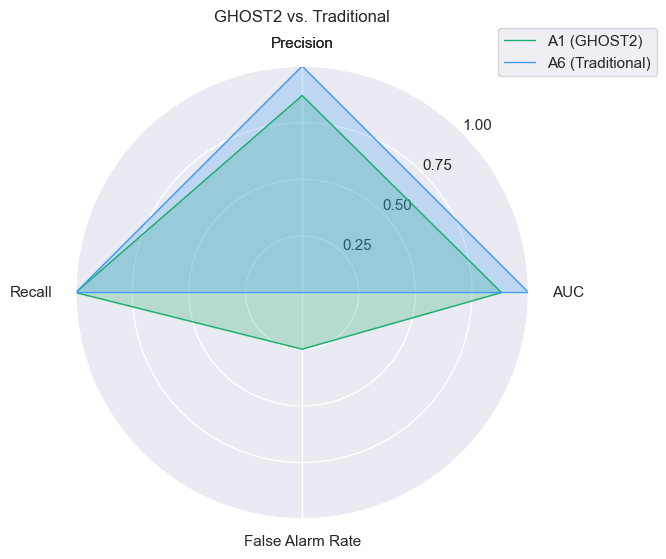
\includegraphics[width=\linewidth]{rahul/comparison.png}
%     \caption{A comparison between A1 (GHOST2), which uses feedforward networks with 9.4\% labels, vs. A6, which uses traditional learners with all the data. Values shown are the medians across 8 datasets. IoU = 0.67}
%     \label{fig:radar}
% \end{figure}





% So far, we have discussed techniques that add in additional data samples to the training set. However, if the original training set is small, as is the case with our datasets, this can lead to the learner over-prioritizing outliers, which can lead to poor performance. We fix this with \textit{label engineering}.


% \subsection{Label Engineering}
% \label{sec:labelengineering}

% Learning algorithms often make assumptions about the data, such as all of it coming from the same distribution. An inherent assumption is also that the labels are correct; but as pointed out by \citet{cordeiro2020survey}, this is often not true. For example, noisy labels can occur when human annotators are present \cite{mcnicol2005primer} and have divergent opinions, as seen in medical images \cite{barkan2021reduce, ma2019blind}. Although our labels were re-checked by the authors of \citet{kang2022detecting}, we assume that some labels are noisy. To rectify the situation, we attempt a simple kind of semi-supervised learning, following Occam's razor. First, given $n$ training samples (and therefore, $n$ labels), we keep $\sqrt{n}$ at random and discard the rest. Next, for each ``unknown'' label, we look at the $\sqrt{\sqrt{n}} = \sqrt[4]{n}$ nearest labels. We take the mode of these labels and assign it as the label for that point. This has the effect of removing outliers in the data. While primitive, our ablation study (of Figure \ref{fig:results})
% confirms that this indeed helps our learning process and improves results. Therefore, we caution researchers to not trust the labels they are given. The details of the number of labels used is given in Table \ref{tab:data}. From the table, we use 58 / (58+554) = 9.5\% labels (which, as we describe later, is $\sqrt{n}$ labels per dataset).




